% vim: fileencoding=utf-8

\documentclass[handout]{beamer}

\usepackage[utf8]{inputenc}
\usepackage[russian]{babel}
\usepackage[T1]{fontenc}
\usepackage{graphicx}
\usepackage{listings} 
\usepackage{xcolor} 
\usepackage{amsmath}

\lstset{%
  language=Python,
  extendedchars={true},
  inputencoding={utf8},
  frame=leftline,
  % framexleftmargin=1cm,
  xleftmargin=0.5cm,
  numbers={left},
  numberstyle={\tiny},
  basicstyle={\ttfamily \scriptsize},
  keywordstyle={\rmfamily \bfseries},
  commentstyle={\rmfamily \itshape},
  tabsize={4},
  showstringspaces=false,
  breaklines=true,
  breakatwhitespace=true,
  escapechar=\%
} 

\usepackage{algpseudocode} 
\usepackage{algorithm} 
\floatname{algorithm}{Алгоритм}

\usepackage{tabularx}

%% Preamble

\usetheme{Madrid}
\usecolortheme{whale}
% \setbeamersize{text margin left=1cm}

%% Title slide

\title[Вывод типов для Python в IDE]{ Вывод типов для языка Python в интегрированной среде разработки }
\author[М.В.~Голубев]{% 
  М.В.~Голубев 63501/13 \\ \vspace{.10cm} 
  {\small научный руководитель} \\ \vspace{.10cm} А.С.~Власовских, ст. разработчик, JetBrains
}

\institute[СПбГПУ]{
  % Институт информационных технологий и управления \\
  % Кафедра компьютерных систем и программных технологи
  \normalsize
  Направление: 230100 --- Информатика и вычислительная техника \\

  Магистерская программа: 230100.68.15 --- Технологии проектирования системного и
  прикладного программного обеспечения
}
\date[20.06.2014]{%
  \\ \vspace{1cm}
  \footnotesize Санкт-Петербургский государственный политехнический университет
}


%% Main content

\begin{document}

\frame{\titlepage}

\begin{frame}
  \frametitle{Проблема}

  В языках с динамической типизацией проверки типов осуществляются только во время исполнения программы.
  \begin{itemize}
      \item Примеры: Python, Ruby, Perl, JavaScript, Clojure и др.
      \item Достоинства:
        \begin{enumerate}
            \item Лаконичный синтаксис без аннотаций типов.
            \item Нет длительного этапа компиляции при разработке.
            \item Больше возможностей метапрограммирования.
        \end{enumerate}
      \item Недостатки:
        \begin{enumerate}
            \item Низкое быстродействие.
            \item \textbf{Нет встроенных средств для статического поиска ошибок типов.}
        \end{enumerate}
  \end{itemize}
    
\end{frame}



\begin{frame}
  \frametitle{Статический анализ}

  Решением является использование в процессе разработки инструментов,
  осуществляющих статический анализ программ для поиска ошибок.

  \begin{itemize}
      \item Пакетные анализаторы: PyLint, PyFlakes
      \item Среды разработки (IDE): \textbf{PyCharm}, PyDev, Wing IDE
  \end{itemize}
    
  Однако из-за недостатка информации точный вывод типов выражений возможен лишь
  в ряде случаев.

\end{frame}

\begin{frame}[fragile]
  \frametitle{Источники информации о типах}

  % \begin{lstlisting}[
    % label={lst:type-sources},
    % gobble=2
  % ]
  % def python_modules(dir_path:str, extension='.py'):
    % """Returns list of Python modules in directory.

    % :type extension: str
    % :type dir_path: str
    % :rtype: list[str]
    % """
    % assert isinstance(extension, str)

    % p = Path(dir_path)
    % result = []
    % for child in p.iterdir():
        % if child.is_file() and child.suffix == extension:
            % result.append(str(child))
    % return result
  % \end{lstlisting}
  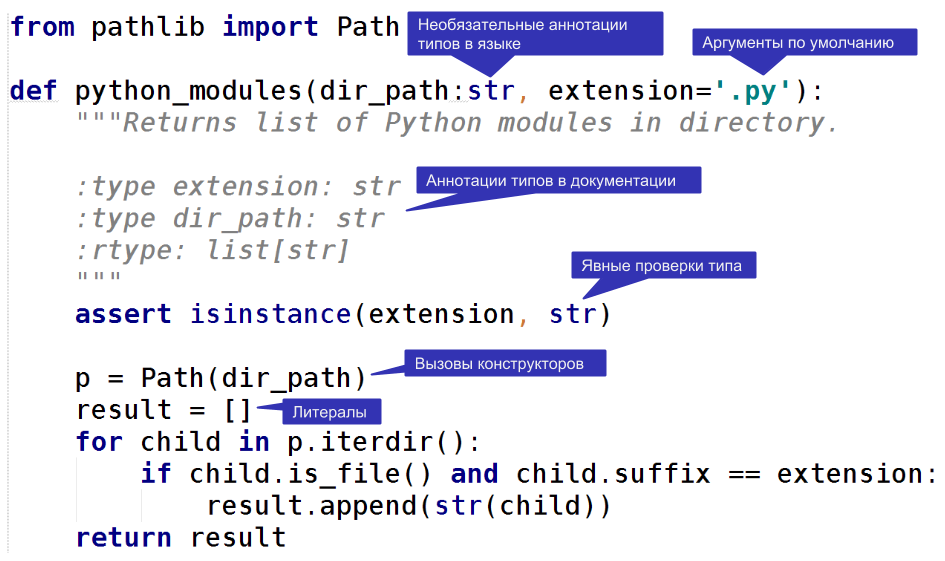
\includegraphics[width=0.9\paperwidth]{fig/type-sources-annotated.png}
    
\end{frame}

\begin{frame}
    \frametitle{Постановка задачи}
    \begin{block}{Задача}
        Разработать метод, при помощи которого можно было бы улучшить существующие
        возможности среды PyCharm по выводу типов в программах на Python.
    \end{block}

    Требования:
    \begin{itemize}
        \item Метод должен быть как можно более точным при, по возможности,
          наибольшей полноте.

        \item Метод должен иметь быстродействие, достаточное для его использования в
          IDE.

        \item Метод должен быть совместим с имеющимся статическим анализом в
          среде PyCharm.
    \end{itemize}

\end{frame}

\begin{frame}[fragile]
  \frametitle{Проблема вывода параметров функций}

  PyCharm может вывести типы параметров функций в следующих случаях:
  \begin{enumerate}
    \item Первый параметр методов \texttt{self}, неявно передаваемый при их
      вызове (30\% всех параметров).

    \item Параметры со значением по умолчанию, если это значение не
      \texttt{None} (1--10\% всех параметров).

    \item Параметры, типы которых указаны в программной документации.

    \item Параметры с явной аннотацией типа (только Python 3).
  \end{enumerate}

  \begin{lstlisting}[
    label={lst:uninferred-types},
    gobble=2
  ]
  def sanitize_url(url):
      sanitized = url.lower()
      if url.endswith('/'):
          sanitized = sanitized[:-1]
      return sanitized
  \end{lstlisting}

  Предполагаемый тип функции: $str \rightarrow str$, однако PyCharm не может вывести ее
тип.

\end{frame}

\begin{frame}[fragile]
  \frametitle{Предлагаемый подход}
  
  \begin{block}{Основная идея}
    Обращениями к методам и полям объекта программист задает неявный контракт на
    его значение. Таким образом, можно подбирать возможные классы для
    параметров функций на основе информации об их атрибутах, используемых в теле
    функции. 
  \end{block}

  \begin{lstlisting}[
    label={lst:uninferred-types},
    emph={lower,endswith},
    emphstyle=\color{blue},
    gobble=2
  ]
  def sanitize_url(url):
      sanitized = url.lower()
      if url.endswith('/'):
          sanitized = sanitized[:-1]
      return sanitized
  \end{lstlisting}

  Ранее подобный подход был описан для языка Smalltalk в работе F.
  Pluquet, A.  Marot, R. Wuyts ``Fast type reconstruction for dynamically
  typed programming languages''.

\end{frame}

\begin{frame}
  \frametitle{Проблема поиска унаследованных атрибутов}
  Предлагаемый подход --- спускаемся от корня в глобальной иерархии классов,
  ищем наиболее общие классы, где есть необходмые атрибуты.

  Пример: ищем класс с атрибутами \texttt{m1} и \texttt{m2}.
  \begin{figure}
    \begin{center}
      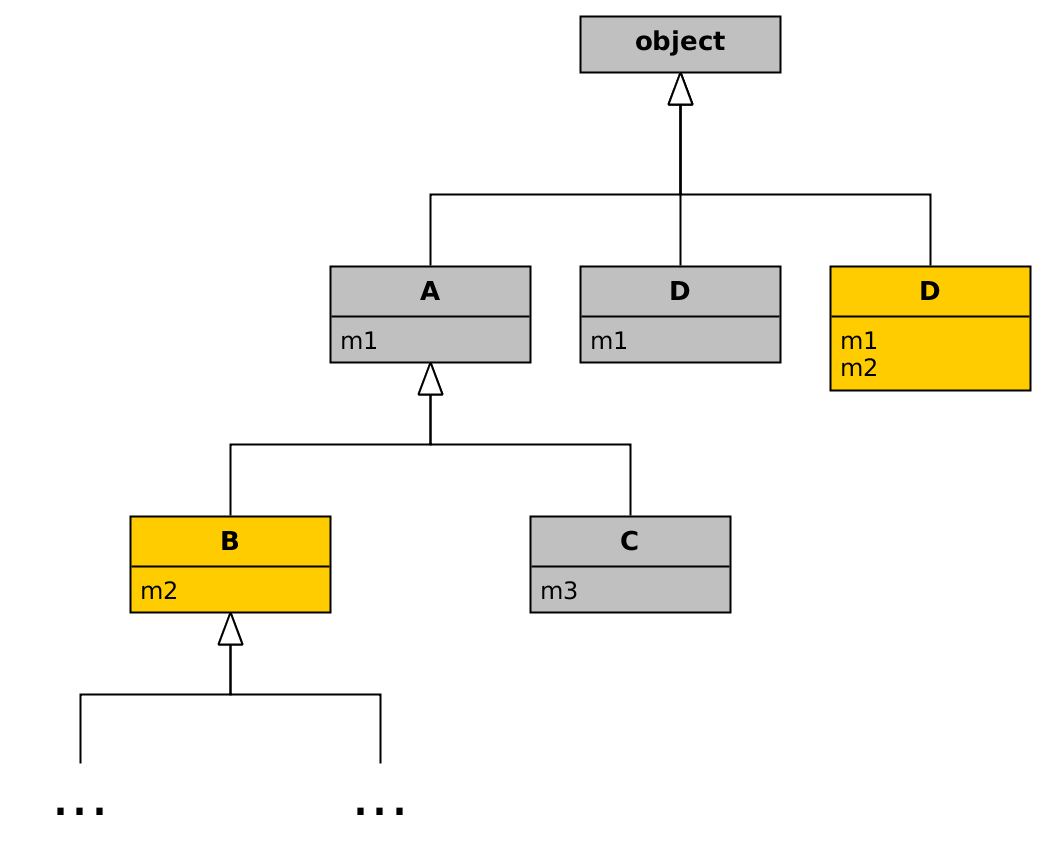
\includegraphics[width=0.6\linewidth]{fig/class-search-example.png}
    \end{center}
  \end{figure}
\end{frame}

\begin{frame}
  \frametitle{Проблема поиска унаследованных атрибутов}
  \framesubtitle{Ограничения существующего подхода}

  Такой подход неприменим в PyCharm:
  \begin{itemize}
    \item В Python возможно множественное наследование между классами.

    \item Требует наличия в памяти всей иерархии классов, что чрезвычайно
      ресурсозатратно (> 1 Гб для больших проектов).
  \end{itemize}

  Для минимизации потребляемой памяти путем выгрузки неиспользуемой информации о
  программе на диск с сохранением скорости поиска в IDE используются
  \emph{индексы}.
  
\end{frame}

\begin{frame}
  \frametitle{Поиск унаследованных атрибутов}
  \framesubtitle{Использование индексов}
  
  Идеальный вариант --- построить индекс $ClassesWithAttributes^*$ вида

  \begin{multline*}
    AttributeName \rightarrow \{class: AttributeName \in \\
  (DeclaredAttributes(class) \cup InheritedAttributes(class)) \}
  \end{multline*}

  Тогда поиск подходящих классов для параметра $p$ сводится к операции

  \[
    suitableClasses_p = \bigcap\limits_{\forall{a} \in AccessedAttributes(p)}
    ClassesWithAttribute^*(a)
  \]
  
\end{frame}

\begin{frame}
  \frametitle{Поиск унаследованных атрибутов}
  \framesubtitle{Использование индексов для поиска классов (продолжение)}

  Индекс $ClassesWithAttribute^*$ не обладает свойством \emph{инкрементальности}.

  \begin{block}{Инкрементальность индекса}
    Инкрементальный индекс при изменении в проекте не требует изменения
    записей в индексе для каких-либо файлов, кроме изменившегося.
  \end{block}

  В индексе $ClassesWithAttribute^*$ изменение какого-либо базового класса
  потребует изменения записей индексов для всех его наследников.
\end{frame}

\begin{frame}
  \frametitle{Поиск унаследованных атрибутов}
  \framesubtitle{Предлагаемое решение}

  Строим более простой индекс $ClassesWithAttribute$
  \begin{multline*}
    AttributeName \rightarrow \{class: AttributeName \in DeclaredAttributes(class) \}
  \end{multline*}

  \begin{enumerate}
    \item На первом шаге алгоритма делаем предвыборку всех классов-кандидатов для
      параметра $p$:  
      \[
        candidateClasses_p = \bigcup\limits_{\forall{a} \in AccessedAttributes(p)}
        ClassesWithAttribute(a)
      \]

    \item Далее ищем унаследованные атрибуты, исключая из множества неподходящие классы
      и кэшируя найденные базовые классы.

    \item На последнем шаге из множества оставшихся классов исключаем те, базовый класс
      которых также находится во множестве.
  \end{enumerate}
\end{frame}


\begin{frame}[fragile]
  \frametitle{Алгоритм}

  \begin{algorithm}[H]
    % \caption{Алгоритм подбора классов по структурному типу.}
    % \label{lst:algorithm-pseudocode}
    \begin{algorithmic}[1]
    \scriptsize
    \Function{SuggestClasses}{$accessedAttributes$}
      \State $candidates \gets \bigcup\limits_{\forall a \in accessedAttributes}
      ClassesWithAttribute(a)$
      \State $suitable \gets \emptyset$
      \While{$candidates \ne \emptyset$}
        \State $class \gets Pop(candidates)$
        \State $bases \gets ResolveBases(class)$
        \State $availableAttributes \gets Attributes(class) \cup \bigcup\limits_{\forall{b} \in bases} Attributes(b)$
        \If{$accessedAttributes \subseteq availableAttributes$}
          \State $suitable \gets suitable \cup \{candidate\}$
        \EndIf
      \EndWhile
      \ForAll{$class \in suitable$}
        \ForAll{$base \in ResolveBases(class)$}
          \If{$base \in suitable$}
            \State $suitable = suitable \setminus \{ class \}$
            \State \textbf{break}
          \EndIf
        \EndFor
      \EndFor
    \State \textbf{return} $suitable$
    \EndFunction
    \end{algorithmic}
  \end{algorithm}

\end{frame}

\begin{frame}
  \frametitle{Прототип}

  \begin{itemize}
      \item Верхняя оценка сложности алгоритма $O((k + n) \cdot n)$, где $n$ ---
        число известных классов, $k$ --- число атрибутов параметра.

      \item Для проверки характеристик предлагаемого подхода был разработан прототип.

      \item Прототип написан на Python и использует модуль \texttt{ast} для
        синтаксического разбора и построения абстрактных синтаксических деревьев
        (AST).

      \item В прототипе сохранено требование независимой индексации отдельных
        модулей.

      \item Первый параметр методов не учитывается при выводе, так как известен
        в PyCharm.

      \item Было проанализировано 60+ проектов на Python.
  \end{itemize}
\end{frame}

\begin{frame}
  \frametitle{Собираемые данные}
  \framesubtitle{Django}

  \begin{table}[H]
    \scriptsize

    \begin{tabularx}{\textwidth}{ |X|X| }
      \hline

      \bfseries Измеряемая характеристика & \bfseries Значение

      \\ \hline

      Число параметров в проекте & 9457 
      \\ \hline
      Параметры без чтений атрибутов & 7378 (78.02\%) 
      \\ \hline
      Параметры с атрибутом, но без выведенного типа & 180 (1.90\%) 
      \\ \hline
      Параметры с одним выведенным типом & 523 (5.53\%) 
      \\ \hline
      Параметры с несколькими выведенными типами & 1376 (14.55\%) 
      \\ \hline

      Максимальное число базовых классов & 7 
      \\ \hline
      Максимальное число с одним из использованных атрибутов & 210 
      \\ \hline
      Максимальное число использованных атрибутов параметра & 11 
      \\ \hline
      Максимальное число предложенных классов & 106 (атрибут \texttt{name}) 
      \\ \hline

      Время вывода всех параметров\footnote{усредненное по результатам пяти запусков} & 688 мс (максимум 15 мс на параметр)
      \\ \hline

      Время вывода всех параметров (кэш базовых классов сбрасывается
      для каждого параметра) & 5104 мс (максимум 19 мс на параметр)
      \\ \hline

    \end{tabularx}
  \end{table}
\end{frame}

\begin{frame}
  \frametitle{Собираемые данные}
  \framesubtitle{Значения для всех проектов}

  \begin{table}[H]
    \scriptsize

    \begin{tabularx}{\textwidth}{ |X|X| }
      \hline

      \bfseries Измеряемая характеристика & \bfseries Значение

      \\ \hline
      Параметры без чтений атрибутов & 81.02\%
      \\ \hline
      Параметры с атрибутом, но без выведенного типа & 3.26\%
      \\ \hline
      Параметры с одним выведенным типом & 3.24\% 
      \\ \hline
      Параметры с несколькими выведенными типами & 12.48\%
      \\ \hline

      Максимальное число базовых классов & 13
      \\ \hline
      Максимальное число с одним из использованных атрибутов & 671 
      \\ \hline
      Максимальное число использованных атрибутов параметра & 33 
      \\ \hline
      Максимальное число предложенных классов & 181 (атрибут \texttt{name}) 
      \\ \hline

      Максимальное время вывода типа параметра & 21 мс
      \\ \hline

      Максимальное время вывода типа параметра (кэш базовых классов сбрасывается
      для каждого параметра) & 38 мс
      \\ \hline

    \end{tabularx}
  \end{table}
\end{frame}

\begin{frame}
  \frametitle{Оценки точности и полноты}

  \begin{itemize}
      \item Точный (\emph{sound}) статический анализ не сообщает о \emph{ложных} ошибках.

      \item Полный (\emph{complete}) статический анализ находит \emph{все} ошибки.
  \end{itemize}

  Ищем ошибку передачи в функцию аргумента неверного типа.

  Параметры, для которых не было найдено ни одного типа, задают верхнюю границу
  полноты метода\footnote{относительно всех учитываемых параметров}:

  \begin{multline*}
    Completeness \le 1 - \bar{R}_{parameters~without~types~inferred} = \\
    \bar{R}_{parameters~with~one~type} + \bar{R}_{parameters~with~more~than~one~type} = \\
    0.032 + 0.124 \approx 15.6\%
  \end{multline*}
    
\end{frame}

\begin{frame}
  \frametitle{Оценки точности и полноты (продолжение)}

  Оценка точности анализа потребовала ручной проверки результатов.

  Было выбрано 100 случайных параметров, для которых было выведено более одного
  типа в проанализированных проектах: 82 случая точных результатов, 40
  случаев полных результатов.


  \begin{align*}
    Soundness& \approx 0.82 \\
    Completeness& \approx 0.40 \times 0.156 = 0.0624
  \end{align*}

  Низкое значение полноты не критично, потому что предложенный метод покрывает
  случаи, где типы не могут быть выведены в PyCharm.
    
\end{frame}

\begin{frame}
  \frametitle{Результаты работы}

  \begin{itemize}
      \item Исследованы существующие подходы к выводу типов в программах на
        динамически типизированных языках.

      \item Изучена реализация механизмов вывода типов в среде PyCharm.

      \item Разработан метод для вывода типов параметров функций в программах на
        Python.

      \item Разработана экспериментальная версия для сбора статистики по
        реальным проектам.

      \item Проведена оценка быстродействия и эффективности предложенного
        подхода: метод удовлетворяет поставленным требованиям.
  \end{itemize}
    
\end{frame}


\begin{frame}
  \frametitle{Направления дальнейшей работы}

  Практические направления:
  \begin{itemize}
    \item Интеграция предложенного подхода в среду разработки PyCharm.
  \end{itemize}

  Теоретические направления:
  \begin{itemize}
      \item Адаптация метода для других языков с динамической типизацией,
        например, Ruby и JavaScript.

      \item Использование подхода для вывода типов локальных переменных.
      
      \item Повышение полноты и точности анализа
        \begin{itemize}
            \item чувствительный к потоку исполнения алгоритм поиска атрибутов
            \item учет использований значения параметра с операторами
            \item получение информации об атрибутах из вызываемых функций
        \end{itemize}

  \end{itemize}
    
\end{frame}
%%%%%%%%%%%%%%%%%%%%%%%%%%%%%%%%%%%%%%%%%%%%%%%%%%%%%%%%%%%%%%%%%%%%%%%%%%%%%%%%

\begin{frame}[fragile]
  \frametitle{Пример ошибки типа}
  \framesubtitle{Обращение к несуществующему методу класса}

  \begin{lstlisting}[
    label={lst:type-error-sample},
    gobble={2},
  ]
  class MyClass(object):
    def method(self):
        print('Success')

  inst = MyClass()
  %\color{red}inst.missing()%

  %\color{red}getattr(inst, ''.join(['m', chr(105), 'ssing']))%()

  %\color{red}exec('inst' + '.missing()')%
  
  del MyClass.method
  %\color{red}inst.method()%

  \end{lstlisting}
    
\end{frame}

% \begin{frame}
  % \frametitle{Иллюстрация работы алгоритма}
  % \begin{figure}
    % \begin{center}
      % \only<1 |handout:1>{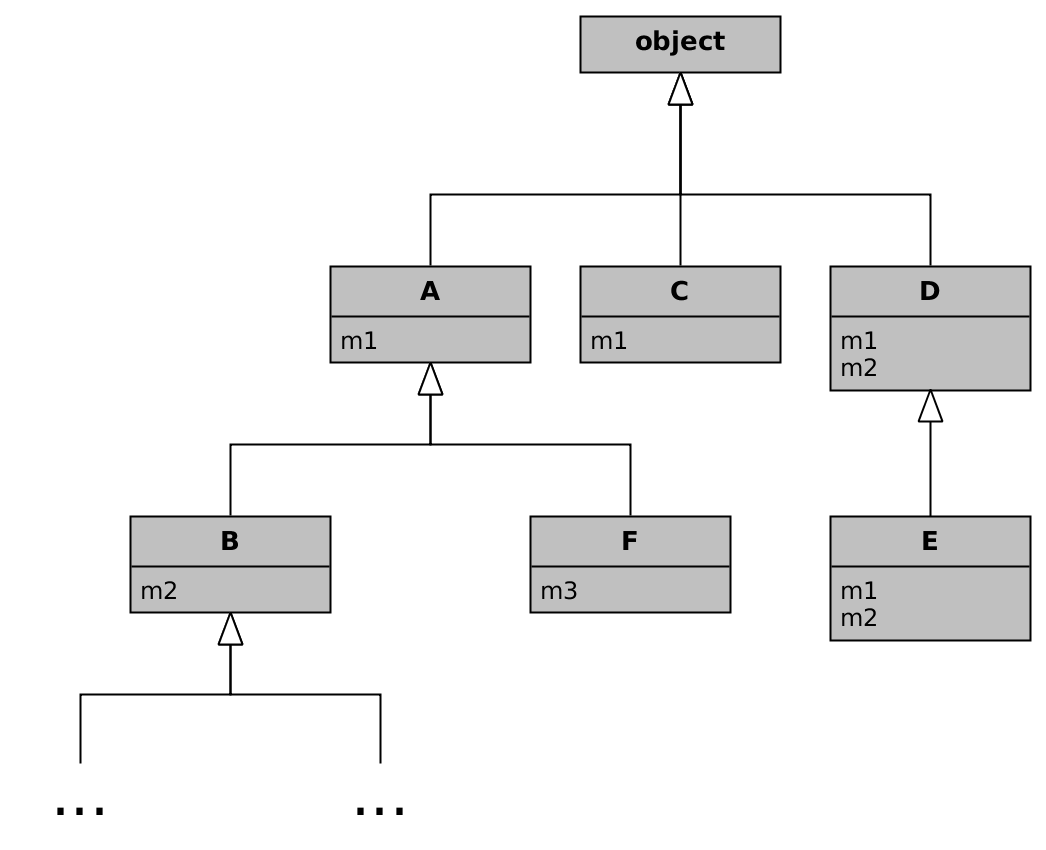
\includegraphics[width=0.7\paperwidth]{fig/class-search-step1.png}}
      % \only<2 |handout:2>{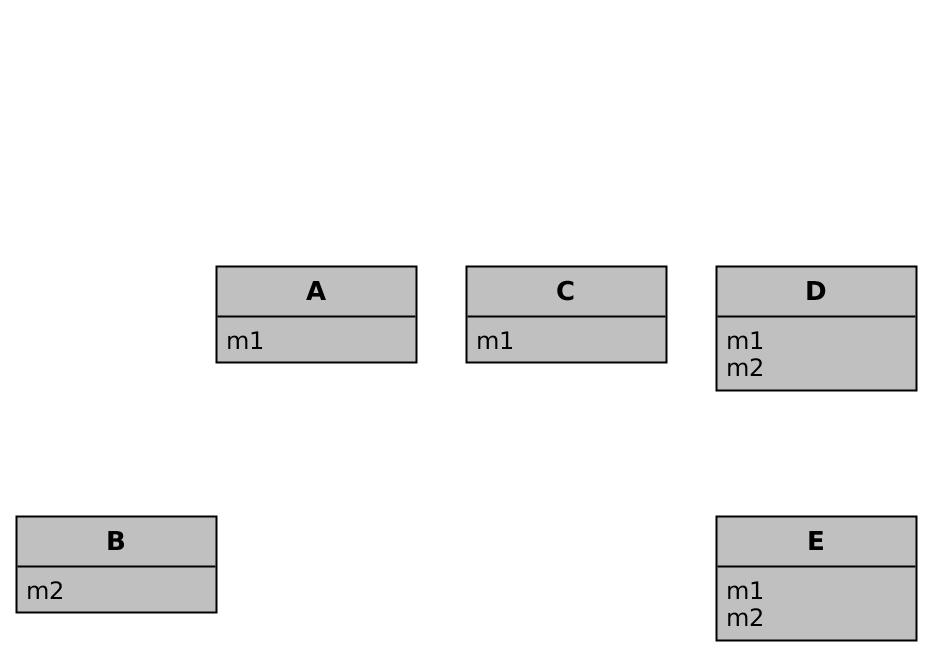
\includegraphics[width=0.7\paperwidth]{fig/class-search-step2.png}}
      % \only<3 |handout:3>{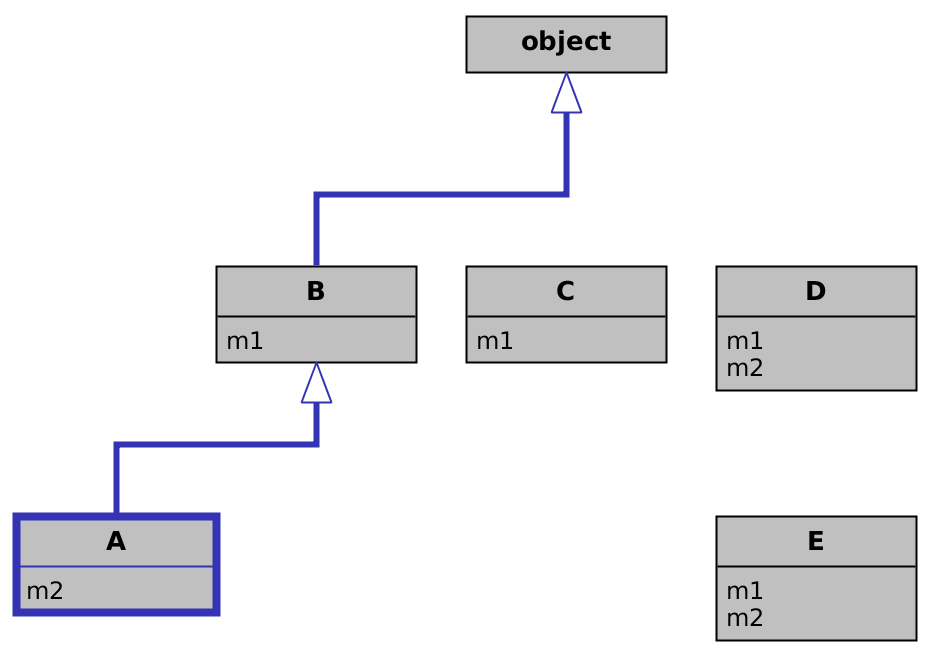
\includegraphics[width=0.7\paperwidth]{fig/class-search-step3.png}}
      % \only<4 |handout:4>{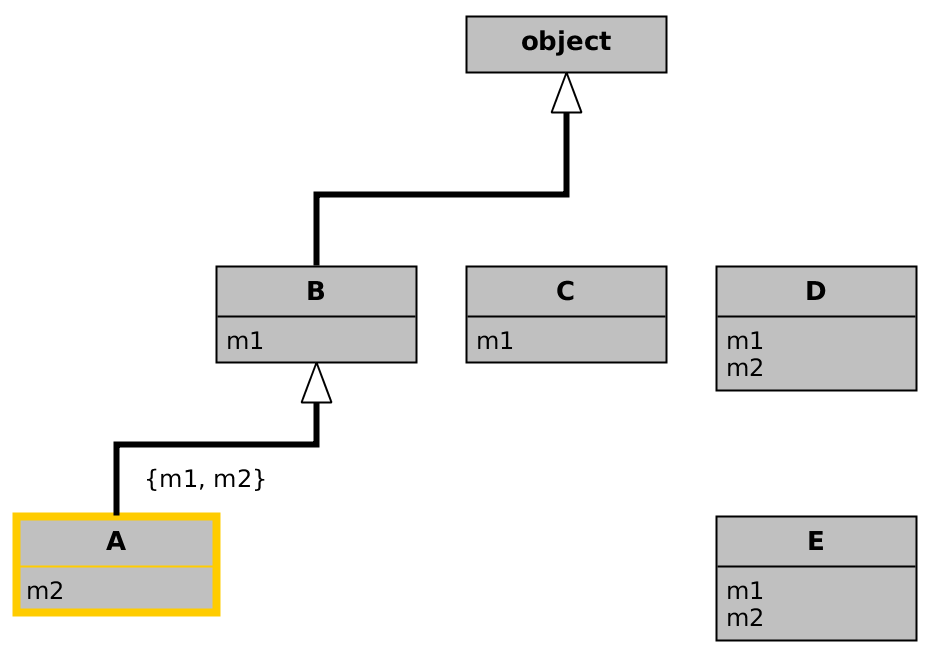
\includegraphics[width=0.7\paperwidth]{fig/class-search-step4.png}}
      % \only<5 |handout:5>{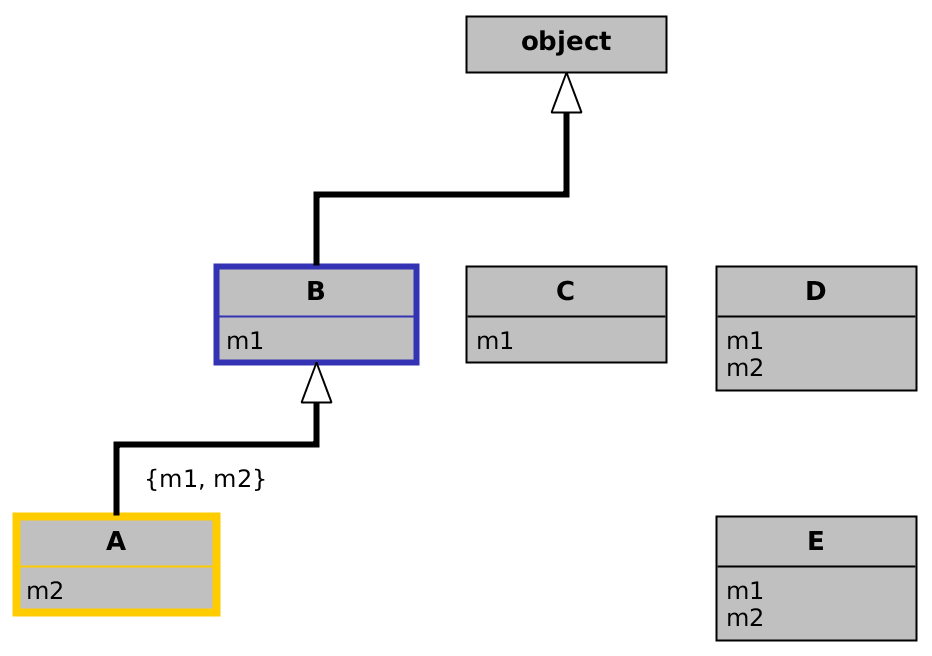
\includegraphics[width=0.7\paperwidth]{fig/class-search-step5.png}}
      % \only<6 |handout:6>{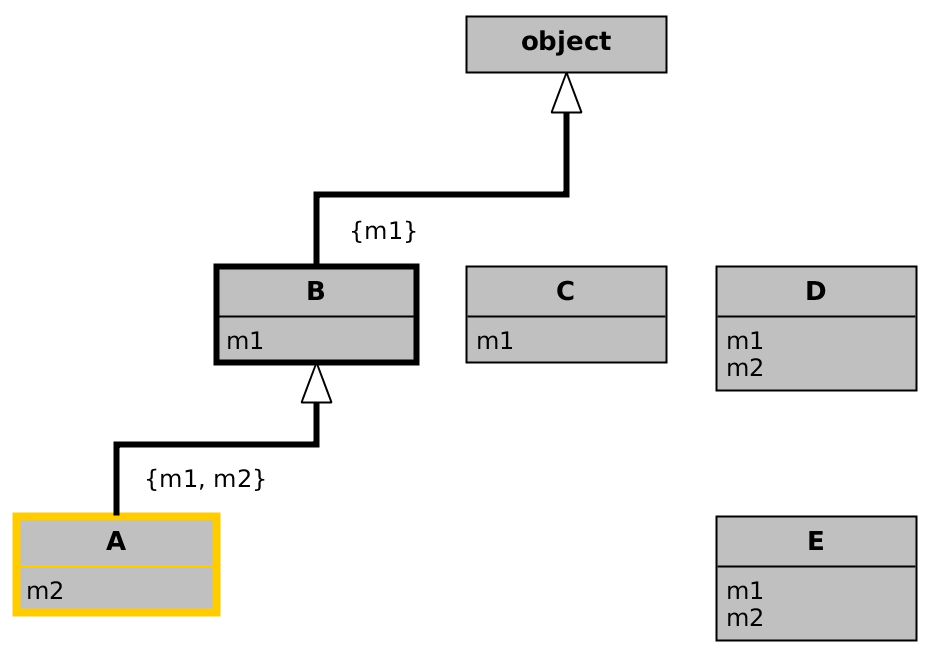
\includegraphics[width=0.7\paperwidth]{fig/class-search-step6.png}}
      % \only<7 |handout:7>{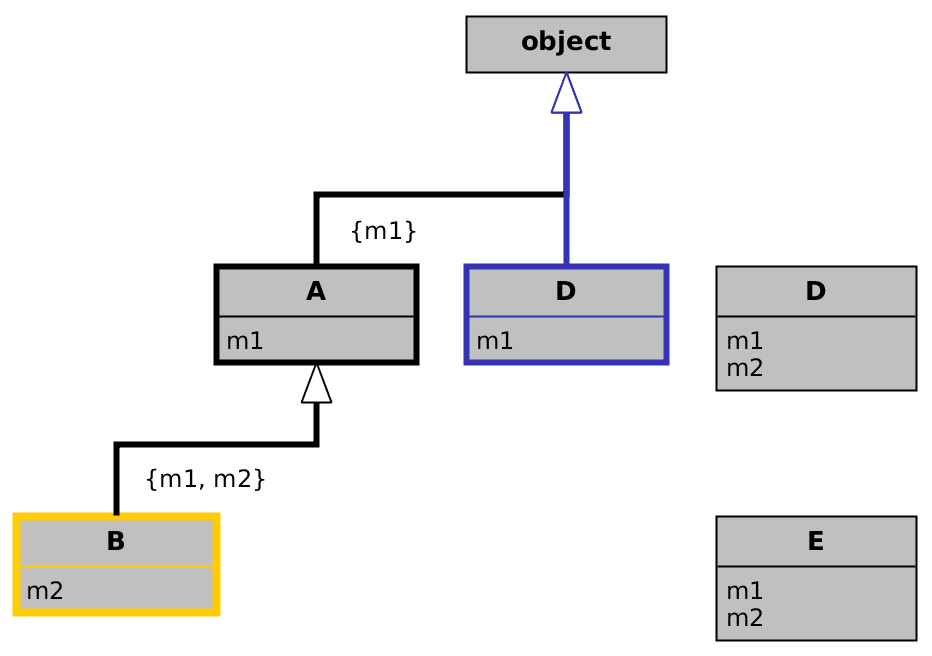
\includegraphics[width=0.7\paperwidth]{fig/class-search-step7.png}}
      % \only<8 |handout:8>{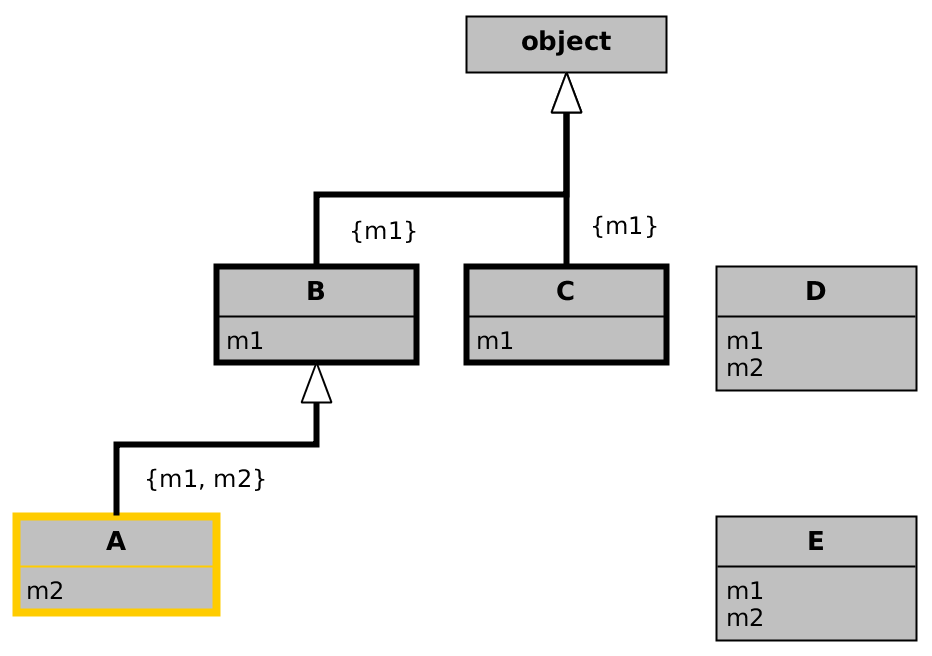
\includegraphics[width=0.7\paperwidth]{fig/class-search-step8.png}}
      % \only<9 |handout:9>{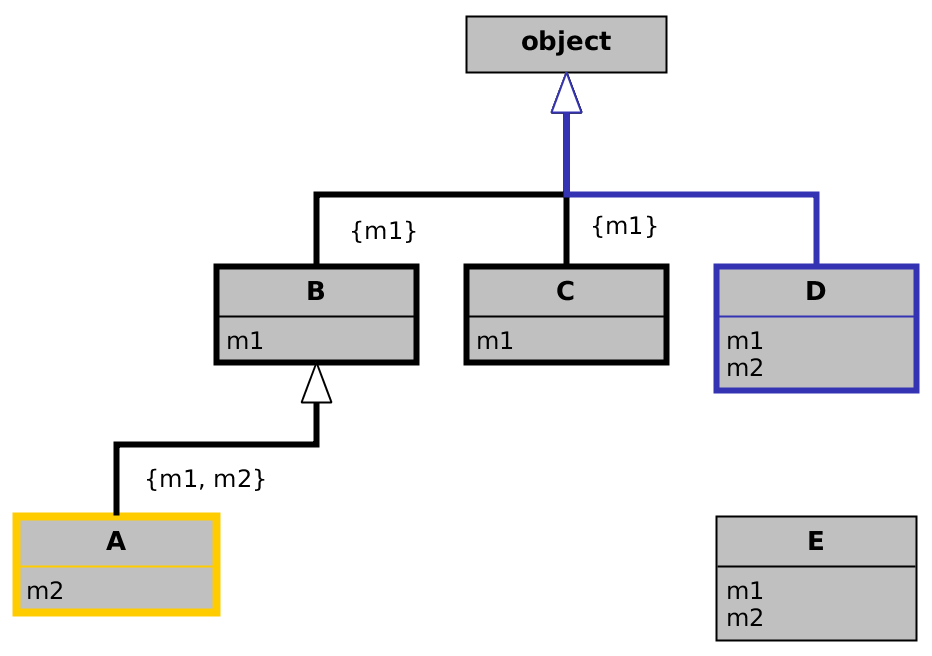
\includegraphics[width=0.7\paperwidth]{fig/class-search-step9.png}}
      % \only<10 |handout:10>{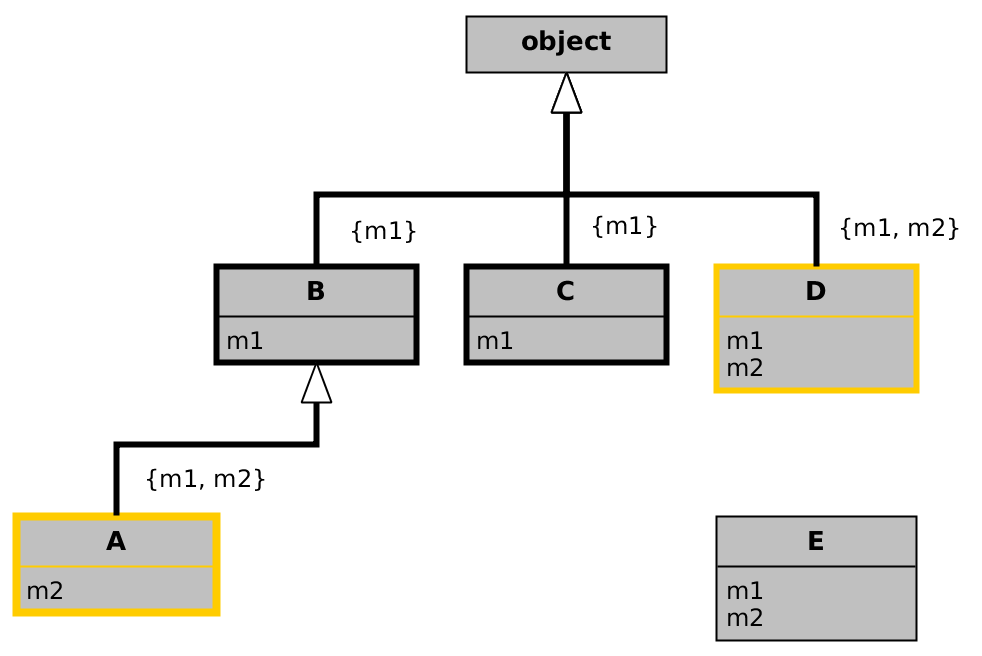
\includegraphics[width=0.7\paperwidth]{fig/class-search-step10.png}}
      % \only<11 |handout:11>{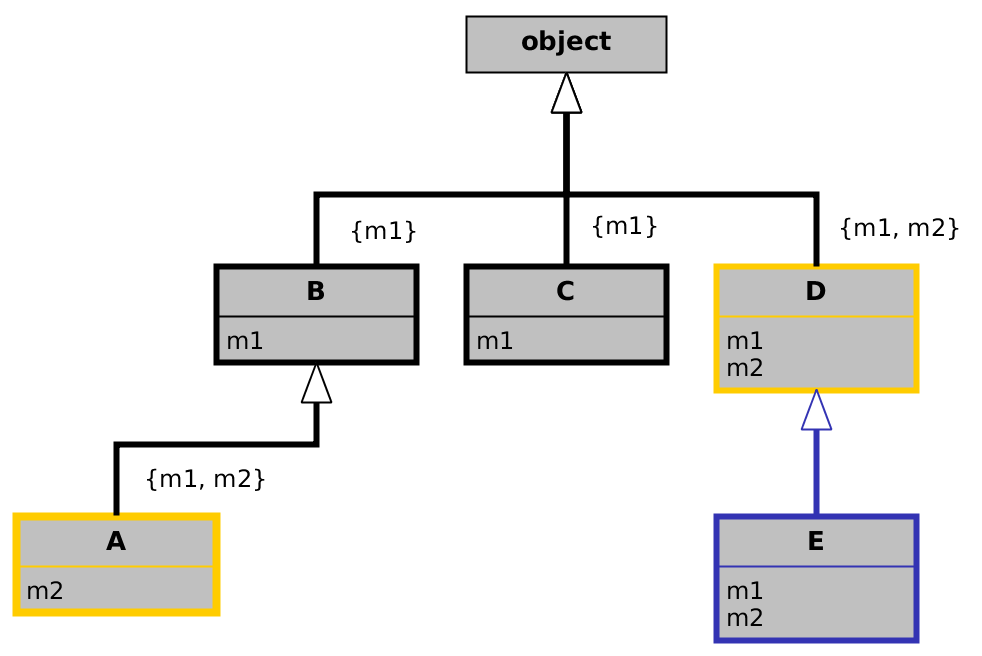
\includegraphics[width=0.7\paperwidth]{fig/class-search-step11.png}}
      % \only<12 |handout:12>{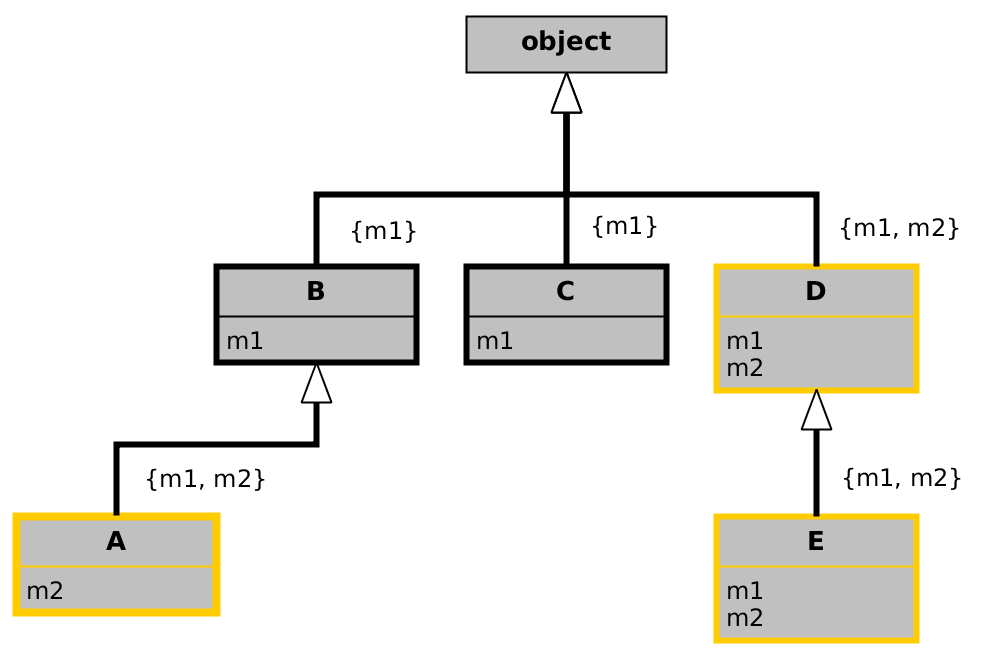
\includegraphics[width=0.7\paperwidth]{fig/class-search-step12.png}}
      % \only<13 |handout:13>{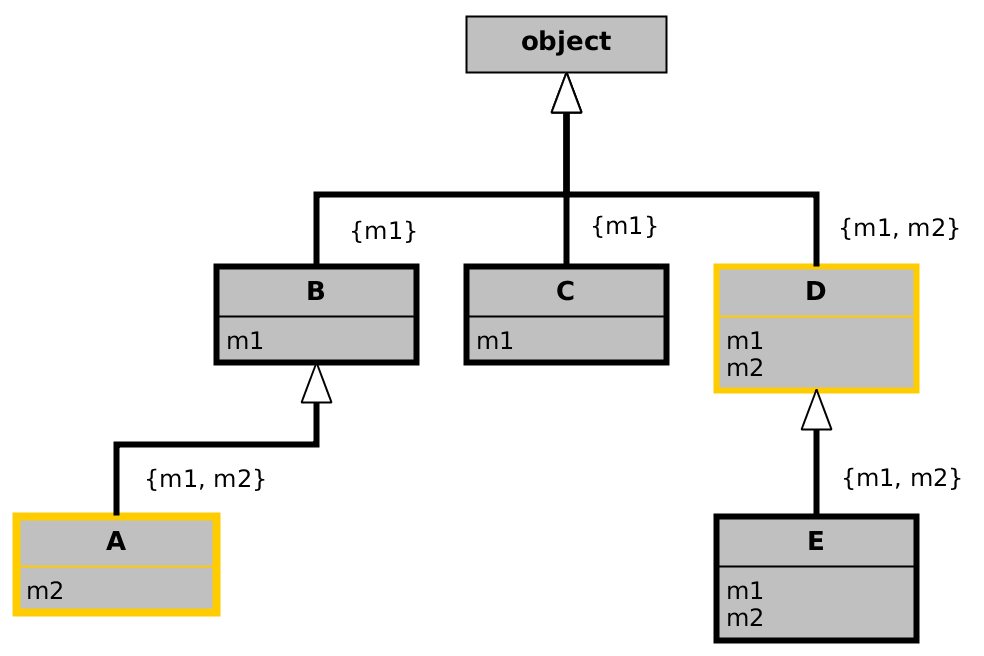
\includegraphics[width=0.7\paperwidth]{fig/class-search-step13.png}}
      % \only<14 |handout:14>{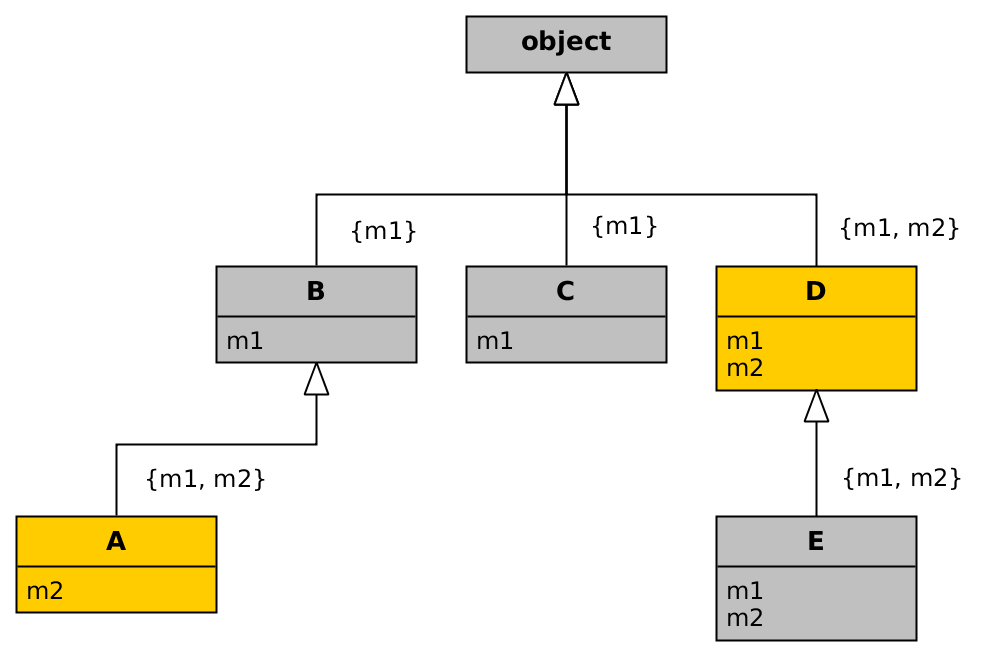
\includegraphics[width=0.7\paperwidth]{fig/class-search-step14.png}}
    % \end{center}
  % \end{figure}
% \end{frame}

\end{document}
